
\subsection{Detaillierte Vegetationsstruktur}

\subsubsection{Geltinger Bucht}

Die Vegetationsbestände in der Geltinger Bucht (dicht bewachsener Standort) setzen sich zusammen aus \textit{Zostera marina} und \textit{Fucus vesiculosus f. balticus}. Das Seegras wuchs bis \unit{30}{\centi\metre} vom Grund mit Deckungsgraden von \unit{70-80}{\%}. In den Wasserschichten \unit{30 bis 60}{\centi\metre} über dem Grund reduzierte sich die Deckung allmählich bis auf \unit{10}{\%}. Nur wenige der schmalen Blattspreiten erstreckten sich darüber hinaus bis zur Oberfläche. Das Wasser war hier etwa \unit{100}{\centi\metre} tief.

Der lose Blasentang ist von kräftigem Wuchs und bedeckt den Boden mit \unit{20}{\%}. Auf \unit{20 und 30}{\centi\metre} Höhe gehen die Pflanzen in die Breite und sorgen für Deckungen von \unit{30}{\%}, darüber verschmälert sich der Blasentang wieder. Große Exemplare erreichten Wuchshöhen von bis zu \unit{50}{\centi\metre}.
In der Mitte der Wassersäule befanden sich mit Deckungsgraden unter einem Prozent freischwimmende filamentöse Algen, die jedoch an zwei Plots Deckungen von \unit{10 und 20}{\%} ausmachten. Die Gesamtdeckung auf den Flächen betrug \unit{90}{\%}, diese wurden vom Grund bis \unit{20}{\centi\metre} Wuchshöhe kartiert, danach nahmen die Deckungen stetig bis zur Oberfläche ab.

\subsubsection{Orther Bucht}

Die Orther Bucht ist zu \unit{30-60}{\%}, im Mittel mit \unit{40}{\%} mit Pflanzen bedeckt. Auf \unit{10}{\centi\metre} Entfernung vom Grund sind \unit{30}{\%} der Wasserschicht bedeckt, darüber ragen nur noch einzelne Stängel von \textit{Potamogeton pectinatus} bis \unit{40}{\centi\metre} Höhe. Das Wasser an diesem Standort ist im Mittel \unit{70}{\centi\metre} tief. Bestandsbildende Art ist \textit{Zannichellia palustris} mit Deckungen von \unit{20-40}{\%}. An einem Plot fehlte die Art, dafür kam hier \textit{Ruppia cirrhosa} mit einer Deckung von \unit{40}{\%} vor. Ebenfalls deckten filamentöse Algen auf \unit{5 bis 10}{\centi\metre} Wuchshöhe zu \unit{20}{\%} den Standort ab. \textit{Potamogeton pectinatus} kam mit Deckungen von bis zu \unit{10}{\%} am Grund vor und verschmälerte sich in der Wassersäule. Von \textit{Chara canescens} und \textit{Tolypella nidifica} wurden vereinzelt Exemplare gefunden.

\subsubsection{Salzhaff}

Das Salzhaff ist zu \unit{80-90}{\%} mit Vegetation bedeckt. Davon machen nicht fest verankerte, filamentöse Algen mit \unit{80}{\%} Deckung auf \unit{5}{\centi\metre} Wuchshöhe den größten Anteil aus. Ihr Anteil reduziert sich in der Wassersäule allmählich bis auf \unit{50}{\centi\metre} Wuchshöhe. \textit{Potamogeton pectinatus} ist mit \unit{30-60}{\%} Deckung die bastandsbildene festsitzende Pflanzenart. Auch sein Anteil reduziert sich allmählich bis \unit{50}{\centi\metre} Wuchshöhe, darüber hinaus reichen wenige Äste bis zur Oberfläche. Das Wasser an diesem Standort ist \unit{80 bis 90}{\centi\metre} tief. Vereinzelt kam auch \textit{Zannichellia palustris} und lose am Grund die Grünalge \textit{Monostroma sp.} vor.

\subsubsection{Spandowerhagener Wiek}

Die gesamte Spandowerhagener Wiek war zu etwa \unit{90}{\%} mit Pflanzen bedeckt, es gab keine ausgedehnten freien Flächen. Den Hauptanteil der Vegetation bildete \textit{Potamogeton pectinatus} mit Deckungsgraden von im Mittel \unit{90}{\%} am Grund, sich allmählich in der Wassersäule reduzierend. Dabei trägt er auf \unit{30}{\centi\metre} Wuchshöhe noch zu einer mittleren Deckung von \unit{50}{\%} bei und wächst bis \unit{50}{\centi\metre} auf. Das Wasser ist \unit{80-85}{\centi\metre} tief. Außerdem kommen \textit{Myriophyllum spicatum} mit \unit{10 bis 20}{\%} Deckung und \textit{Potamogeton perfoliatus}, auf einigen Plots mit bis zu \unit{10}{\%} Deckung vor. \textit{Myriophyllum spicatum} bedeckt mit einem Grund-Abstand von \unit{10 und 20}{\centi\metre} noch \unit{10 bzw. 5}{\%} der jeweiligen Wasserschichten, nur vereinzelte Halme wachsen bis \unit{50}{\centi\metre} auf. \textit{Potamogeton perfoliatus} hingegen nimmt nur bis auf \unit{10}{\centi\metre} relevante Deckungen ein, darüber hinaus gehen wenige Zweige bis \unit{70}{\centi\metre} Wuchshöhe. Auf 2 Plots wurde auch mit \unit{10 bzw. 20}{\%} Anteil in der \unit{5 bis 10}{\centi\metre} -Wasserschicht \textit{Zannichellia palustris} gefunden und es gab wenige vereinzelte Exemplare von \textit{Najas marina}.





\begin{figure}[!htb]
\centering
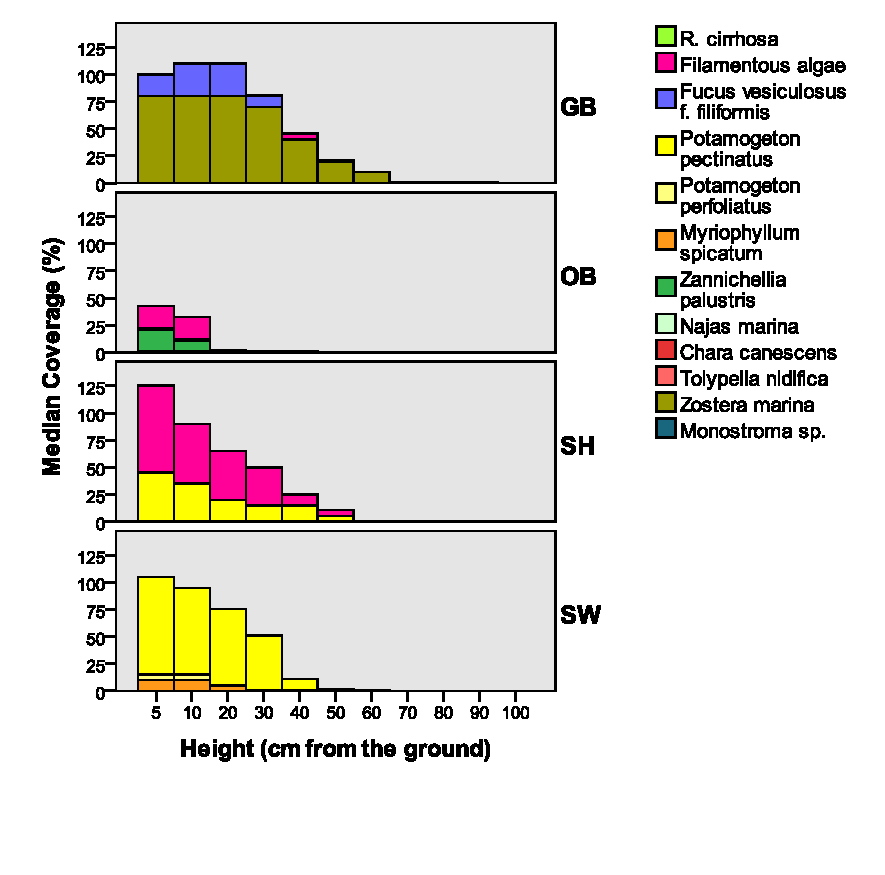
\includegraphics[0.90\textwidth]{images/Wuchshoehenkartierung/salzgradient_gross1.eps}
\caption[Höhenstufenkartierung an den Stationen des Salzgradienten (+M)]{Deckungen aller Arten auf Höhenstufen vom Grund bis zur Oberfläche an den dicht bewachsenen Standorten entlang des Salzgradienten; GB = Geltinger Bucht, OB = Orther Bucht; SH = Salzhaff; SW = Spandowerhagener Wiek}
\label{fig:wuchshoehen_salzgradient_1}
\end{figure}
\\
\begin{figure}[!htb]
\centering
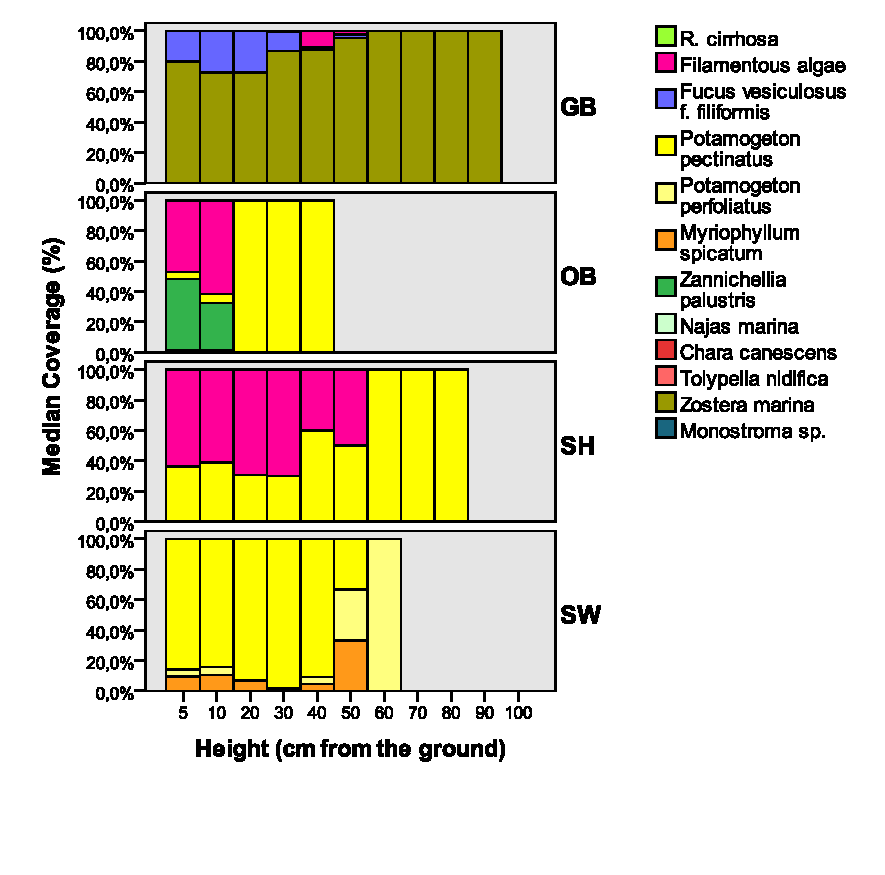
\includegraphics[0.90\textwidth]{images/Wuchshoehenkartierung/salzgradient_gross2.eps}
\caption[Prozentuale Höhenstufenkartierung an den Stationen des Salzgradienten (+M)]{Prozentuale Deckungen aller Arten, bezogen auf die Gesamtdeckung auf jeder Höhenstufe an den dicht bewachsenen Standorten entlang des Salzgradienten; GB = Geltinger Bucht, OB = Orther Bucht; SH = Salzhaff; SW = Spandowerhagener Wiek}
\label{fig:wuchshoehen_salzgradient_2}
\end{figure}

\FloatBarrier


\subsection{Deckung und PVI}

Zum Zeitpunkt der Probenahmen entlang des Salzgradienten waren sowohl die Deckung als auch das PVI an allen vegetationsarmen Untersuchungsgruppen sehr gering. Maximal \unit{2}{\%} der Fläche wurden von Phytobenthos eingenommen und es machte maximal \unit{0,3}{\%} der Wassersäulen aus.

Bei Betrachtung aller vegetationsdominierten Stationen des Salzgradienten im Vergleich zeigt sich, dass es 3 verschiedene Kategorien von Vegetationsbeständen gab. In die erste Kategorie fallen die Orther Bucht und die Griebener Bucht. Diese zeigten Deckungsgrade von \unit{40-60}{\%}. Auch ihre pflanzliche Zusammensetzung ist sich ähnlich. Es gibt grundrasenbildende Arten (\textit{Zannichellia palustris} in der Orther Bucht und\textit{ Ruppia cirrhosa} in der Griebener Bucht) sowie das höher aufwachsende Laichkraut \textit{Potamogeton pectintus} und dazwischen Matten aus fädigen Algen. In dem verhältnismäßig flachen Wasser von \unit{60-70}{\centi\metre} werden PVI-Werte von im Mittel \unit{5}{\%} erreicht. Das Maximum waren \unit{14,4}{\%} in der Orther Bucht.

Die Geltinger Bucht, das Salzhaff und die Spandowerhagener Wiek bilden die zweite Kategorie mit wesentlich höheren Deckungsgraden von \unit{80-95}{\%} und ebenfalls hohen PVI-Werten von \unit{20-30}{\%}. Diese Standorte befinden sich auch in etwas tieferem Wasser (\unit{80-110}{\centi\metre}). Die Geltinger Bucht und die Spandowerhagener Wiek sind sich auch in ihrer Vegetationsstruktur ähnlich. Beide beherbergen Makrophyten, die weit in die Wassersäule hineinreichen und auch in größerem Abstand vom Grund noch hohe Deckungsgrade verursachen. In der Geltinger Bucht ist dies \textit{Zostera marina} und in der Spandowerhagener Wiek sind es Parvopotamiden und \textit{Myriophyllum spicatum}. Im Salzhhaff hingegen werden die hohen Deckungsgrade und pflanzlichen Anteile in der Wassersäule neben dem hoch aufwachsenden \textit{Potamogeton pectintus} zu einem großen Teil von filamentösen Algen verursacht.

Die dritte Kategorie nimmt der Vitter Bodden ein. Bei einer Bedeckung von \unit{100}{\%} ist der Anteil des Phytobenthos an der Wassersäule mit \unit{8-17}{\%} deutlich weniger als bei den 3 zuvor genannten Standorten. Grund hierfür ist die dichte Bedeckung mit \textit{Fucus vesiculosus}, welcher zwar hohe Deckungsgrade verursacht, aber nicht weit in die etwa \unit{83}{\centi\metre} tiefe Wassersäule hineinreicht.



\begin{figure}[!htb]
\centering
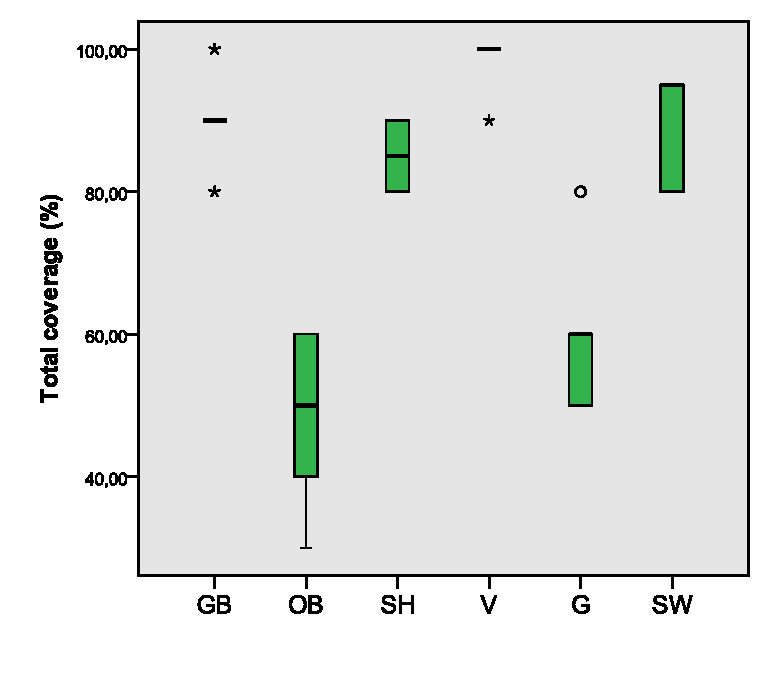
\includegraphics[width=0.80\textwidth]{images/total_cover/cover_salzgradient.eps}
\caption[Bedeckung mit Makrophyten an Standorten entlang des Salzgradienten]{Gesamtbedeckung der Plots mit Makrophyten an den dicht bewachsenen Standorten entlang des Salzgradienten; GB = Geltinger Bucht, OB = Orther Bucht; SH = Salzhaff; SW = Spandowerhagener Wiek}
\label{fig:cover_salzgradient}
\end{figure}

\begin{figure}[!htb]
\centering
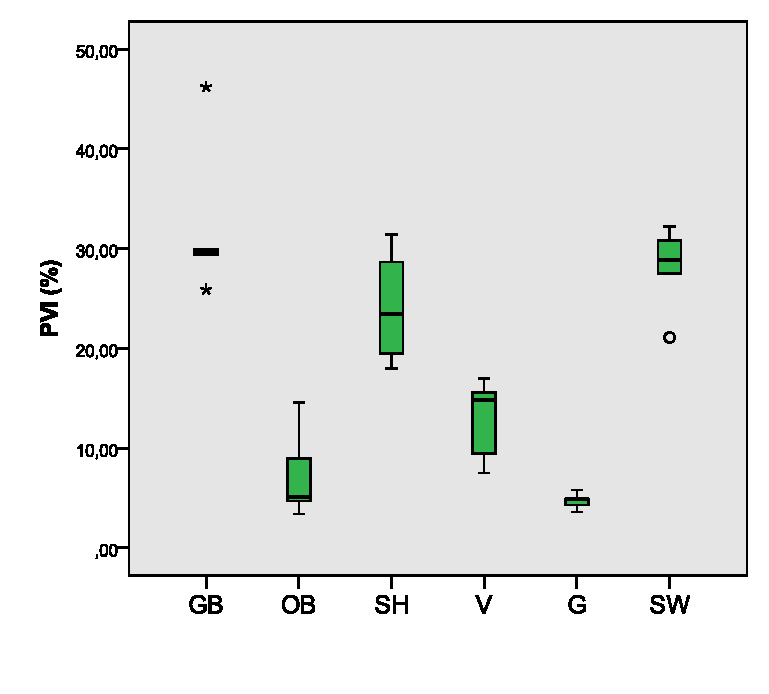
\includegraphics[width=0.80\textwidth]{images/pvi/pvi_salzgradient.eps}
\caption[PVI an Standorten entlang des Salzgradienten]{Anteil des Phytobenthos an der Wassersäule (PVI nach \cite{jeppesen_1998}) an den dicht bewachsenen Standorten entlang des Salzgradienten; GB = Geltinger Bucht, OB = Orther Bucht; SH = Salzhaff; SW = Spandowerhagener Wiek}
\label{fig:pvi_salzgradient}
\end{figure}



\begin{table}[!htb]
\centering
\caption[Deskriptive Statistik, Deckung und PVI entlang des Salzgradienten]{Deskriptive Statistik zu Deckung und PVI an Standorten entlang des Salzgradienten; MAD = Mittlere Abweichung vom Median}
\begin{tabular}{llllll}
\toprule
Category & Location 							& \multicolumn{2}{l}{Total Cover} & \multicolumn{2}{l}{PVI}\\
		 &											& Median	& MAD			  & Median	& MAD\\
\midrule
\multirow{6}{*}{Dense Vegetation}& Geltinger Bucht	& 90.00		& 4.00			  & 29.60	& 4.16\\
								 & Orther Bucht		& 50.00		& 10.00			  & 5.10	& 3.10\\
								 & Salzhaff			& 85.00		& 5.00			  & 23.35	& 4.58\\
								 & Vitter Bodden	& 100.00	& 2.00			  & 14.80	& 3.12\\
								 & Griebener Bucht	& 60.00		& 8.00			  & 4.90	& 0.56\\
								 & Spandowerhagener Wiek & 95.00 & 6.00			  & 28.90	& 2.88\\
\midrule
\multirow{5}{*}{Sparse Vegetation}&Geltinger Bucht	& 2.00		& 0.00			  & 0.18	& 0.00\\
								 & Orther Bucht		& 2.00		& 				  & 0.30\\
								 & Salzhaff			& 0.50		& 0.00			  & 0.10	& 0.00\\
								 & Vitter Bodden	& 0.50		& 0.00			  & 0.00	& 0.00\\
								 & Griebener Bucht	& 2.50		& 1.30			  & 0.33	& 0.01\\
\bottomrule
\end{tabular}
\label{tab:statistik_salzgradient_Deckung,PVI}
\end{table}
\FloatBarrier



\subsection{Sediment}

\subsubsection{Geltinger Bucht}

Das Sediment am dicht mit Phytobenthos besiedelten Standort ist mäßig sortiert und die Verteilungskurve etwas in den grobkörnigen Bereich verschoben. Feinsand und Mittelsand haben mit \unit{45 und 27,5}{\%} den größten Anteil am Gesamt-Korngrößenspektrum. Mit \unit{9 und 8,3}{\%} sind auch sehr grobe und grobe Sande im Sediment enthalten und mit je etwa \unit{5}{\%} sind Feinsand und Ton-/Siltfraktionen vertreten. Der Median der Korngrößenverteilung beträgt $ \Phi $ = 2,1 und der organische Gehalt \unit{1,4}{\%}.

Das Sediment der kaum mit Phytobenthos besiedelten Untersuchungsgruppe war besser sortiert als die der dicht besiedelten Gruppe. Feinsande und Mittelsande hatten hier einen größeren Anteil von \unit{53 und 34}{\%}. Sehr grober Sand war fast nicht und grober Sand nur zu \unit{3}{\%} enthalten. Es waren weniger feine Sande (\unit{2,5}{\%}) aber dafür mit etwa \unit{7}{\%} mehr Ton und Silt enthalten. Der Organische Gehalt ist mit \unit{0,7}{\%} geringer als bei den Sedimenten der dicht mit Seegras und \textit{Fucus vesiculosus} besiedelten Fläche.



\subsubsection{Orther Bucht}

Auf der Phytobenthos-dominierten Untersuchungsfläche ist das Sediment sehr gut sortiert und die Feinsandfraktion dominiert mit \unit{72}{\%}. Daneben kommen zu \unit{16 und 7}{\%} sehr feine und Mittelsande vor. Der Anteil der \unit{<63}{\mu\metre}-Fraktion beträgt hier nur \unit{3}{\%}. Insgesamt ist die Verteilungskurve leicht linksschief (in den feinkörnigen Bereich verschoben) und der Median der Korngröße beträgt $ \Phi $ = 2,6. Der organische Gehalt des Sedimentes ist mit \unit{0,5}{\%} sehr gering.

Das Sediment der vegetationsreichen Untersuchungsgruppe hingegen ist weniger gut sortiert. Mit \unit{62}{\%} ist der Feinsand ebenfalls die am meißten vertretene Korngrößenfraktion, jedoch ist auch der Anteil des Mittelsandes mit etwa \unit{18}{\%} höher. Der Median der Korngröße beträgt $ \Phi $ = 2,5. 

\subsubsection{Salzhaff}

Hier sind sich die Korngrößenfraktionen der dicht und spärlich besiedelten Untersuchungsflächen ähnlich. Die Sedimente sind gut sortiert. Mit \unit{63,5}{\%} (vegetationsarme Gruppe) bzw. \unit{72}{\%} (vegetationsreiche Gruppe) dominieren sehr feine Sande. Daneben kommen Silte und Tone mit \unit{10 bis 12}{\%} sowie Feinsande mit  \unit{15-25}{\%} vor. Im wenig besiedelten Bereich ist der Anteil der Silte und Tone geringer und der Anteil der Feinsande deutlich höher als im dicht besiedelten Bereich. Mittel-bis Grobsande haben keine Bedeutung in den  Korngrößenverteilungen beider Gruppen. Der Median der Korngröße ist in der dicht besiedelten Gruppe mit $ \Phi $ = 3,5 etwas höher als der der spärlich besiedelten Gruppe ($ \Phi $ = 3,4). Das bedeutet, dass Sediment ist in der dicht besiedelten Gruppe etwas feiner. Der organische Gehalt der Sedimente beträgt \unit{1,2 und 0,8}{\%}. Er ist in der dicht besiedelten Untersuchungsgruppe etwas höher. 


\subsubsection{Spandowerhagener Wiek}

In der durchgängig von dichter Vegetation geprägten Spandowerhagener Wiek war das Sediment gut sortiert und die Korngrößenverteilung annähernd symmetrisch. Mit \unit{72,5}{\%} dominiert der Anteil der Feinsandfraktion. 
Daneben haben Mittelsande, sehr feine Sande und Silte / Tone mit \unit{17}{\%}, \unit{6}{\%}, und \unit{3}{\%} ihre jeweiligen Anteile am Sediment. Der Median der Korngrößenverteilung liegt bei $ \Phi $ = 2,4 und der organische Gehalt beträgt \unit{0,9}{\%}.

\begin{table}[!htb]
\centering
\caption[Deskriptive Statistik zu den Korngrößenverteilungen entlang des Salzgradienten]{Deskriptive Statistik zu den Korngrößenverteilungen an den Standorten entlang des Salzgradienten; MAD = Mittlere Abweichung vom Median; +M = dichte Vegetation, -M = spärliche Vegetation; Kennwerte aus den obersten \unit{2}{\centi\metre} des Sedimentkörpers}
\begin{tabular}{lcrrrr}

\toprule

\multicolumn{1}{c}{Location}  & \multicolumn{1}{c}{Category} & \multicolumn{1}{c}{Med Grain Size} & \multicolumn{1}{c}{Sorting} & \multicolumn{1}{c}{< \unit{63}{\mu\metre}} & \multicolumn{1}{c}{AFDW}\\

& 	& \multicolumn{1}{c}{$ (\Phi) $} & & \multicolumn{1}{c}{(\%)} & \multicolumn{1}{c}{(\% DW)}\\

\midrule
\multirow{2}{*}{Geltinger Bucht} & +M & 2.12 & 0.71 & 4.94 & 1.42\\
								 & -M & 2.24 & 0.54 & 6.88 & 0.72\\
\midrule
\multirow{2}{*}{Orther Bucht} & +M  & 2.57 & 0.35 & 3.03 & 0.52\\
							& -M  & 2.46 & 0.41 & 4.00 & 0.55\\
\midrule
\multirow{2}{*}{Salzhaff} & +M & 3.47 & 0.35 & 12.15 & 1.21\\
						& -M & 3.37 & 0.40 & 10.45 & 0.78\\
\midrule
\multirow{2}{*}{Vitter Bodden} & +M & 2.23 & 0.54 & 6.04 & 1.23\\
								& -M & 1.89 & 0.56 & 5.56 & 0.91\\
\midrule
\multirow{2}{*}{Griebener Bucht} & +M & 3.61 & 0.95 & 28.31 & 4.19\\
								& -M & 3.42 & 0.67 & 10.23 & 1.43\\
\midrule
\multirow{1}{*}{Spandowerhagener Wiek} & +M & 2.44 & 0.36 & 2.84 & 0.93\\
\bottomrule

\end{tabular}
\label{tab:statistik_salzgradient_sedimentparameter}
\end{table}
\\


\begin{figure}[!htb]
\centering
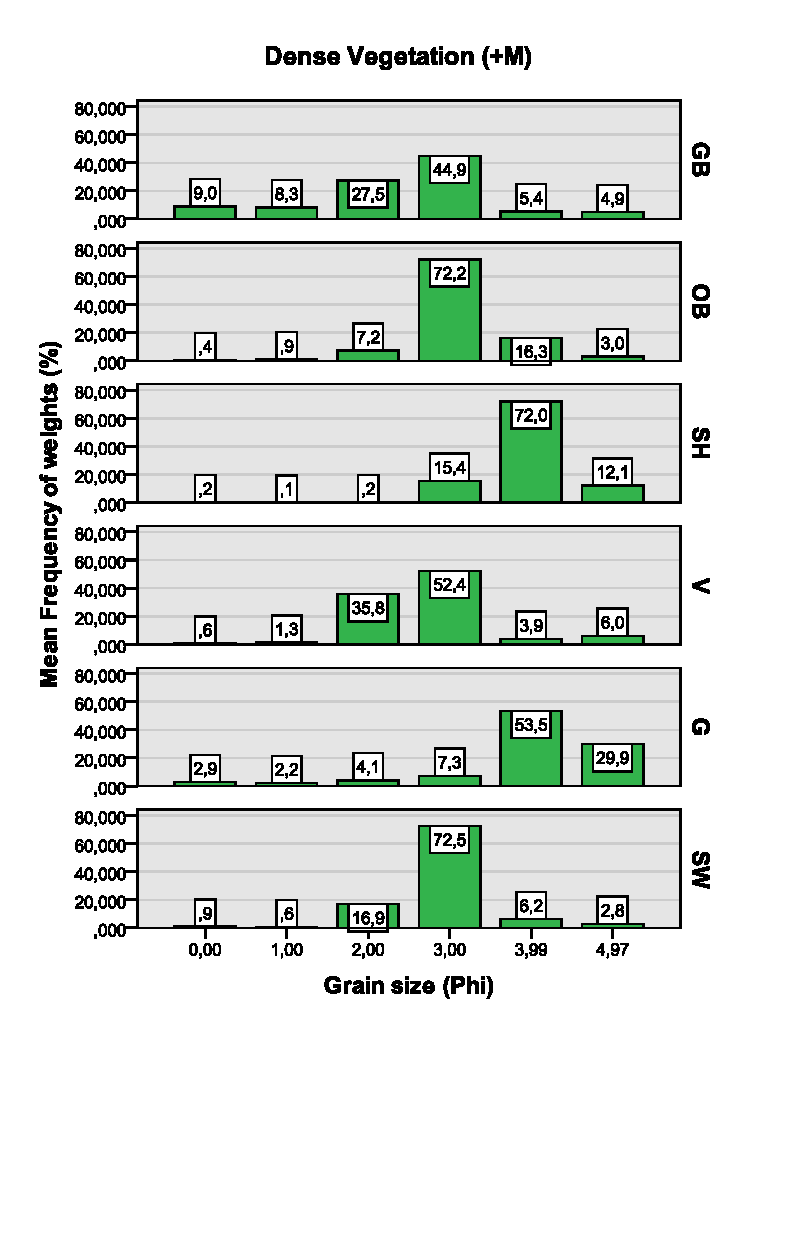
\includegraphics[trim = 0mm 35mm 0mm 0mm, clip, width=0.90\textwidth]{images/grainsize/korngroessenverteilungen_sg1.eps}
\caption[Korngrößenverteilungen entlang des Salzgradienten (+M)]{Korngrößenverteilungen an dicht bewachsenen Standorten entlang des Salzgradienten (+M); GB = Geltinger Bucht, OB = Orther Bucht; SH = Salzhaff; V = Vitter Bodden (5.7.2013), G = Griebener Bucht (30.7.2013), SW = Spandowerhagener Wiek}
\label{fig:korngrössen_salzgradient_+m}
\end{figure}

\begin{figure}[!htb]
\centering
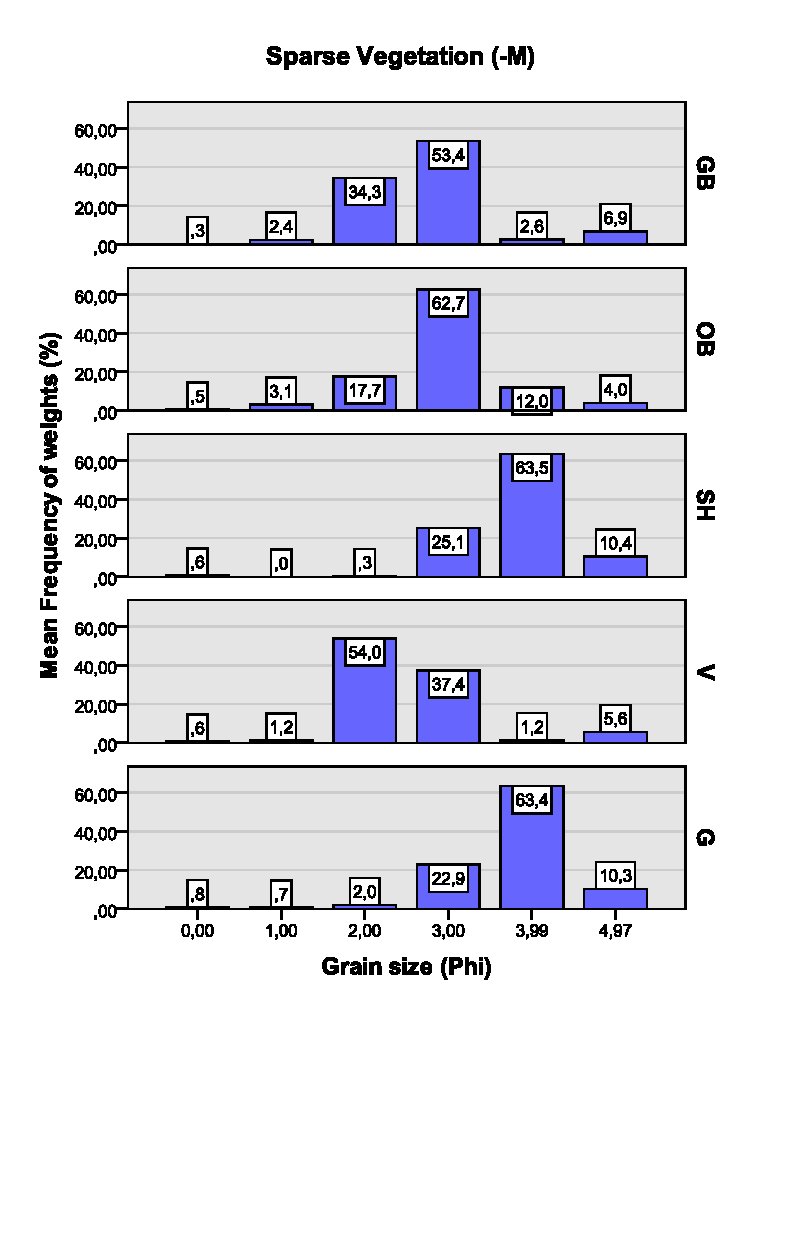
\includegraphics[trim = 0mm 35mm 0mm 0mm, clip, width=0.90\textwidth]{images/grainsize/korngroessenverteilungen_sg2.eps}
\caption[Korngrößenverteilungen entlang des Salzgradienten (-M)]{Korngrößenverteilungen an spärlich bewachsenen Standorten entlang des Salzgradienten (-M); GB = Geltinger Bucht, OB = Orther Bucht; SH = Salzhaff; V = Vitter Bodden (5.7.2013), G = Griebener Bucht (30.7.2013), SW = Spandowerhagener Wiek}
\label{fig:korngrössen_salzgradient_-m}
\end{figure}

\begin{figure}[!htb]
\centering
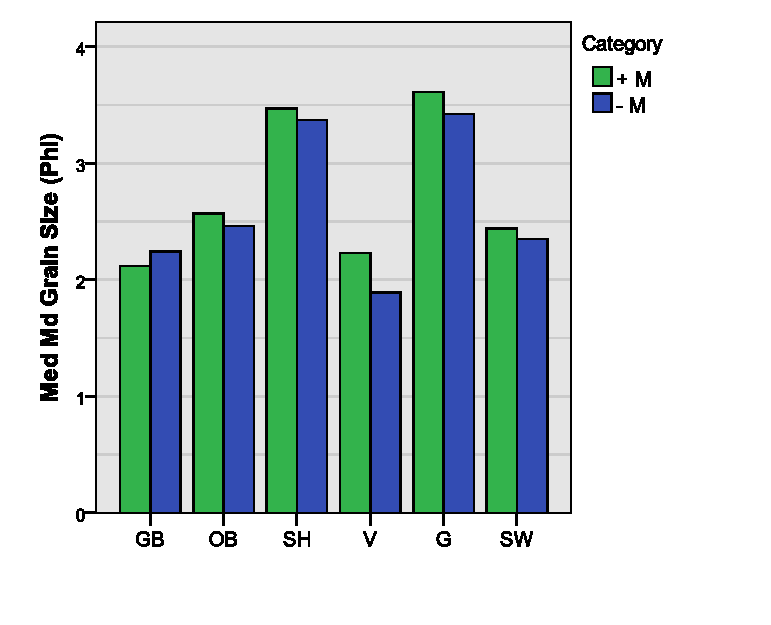
\includegraphics[width=0.75\textwidth]{images/salzsedimentauswertung/bar_mgsize.eps}
\caption[Median der Korngrößen an Stationen des Salzgradienten]{Median der Korngrößen an Stationen des Salzgradienten; GB = Geltinger Bucht, OB = Orther Bucht; SH = Salzhaff; V = Vitter Bodden (5.7.2013), G = Griebener Bucht (30.7.2013), SW = Spandowerhagener Wiek}
\label{fig:sg:mittlere_kg}
\end{figure}

\begin{figure}[!htb]
\centering
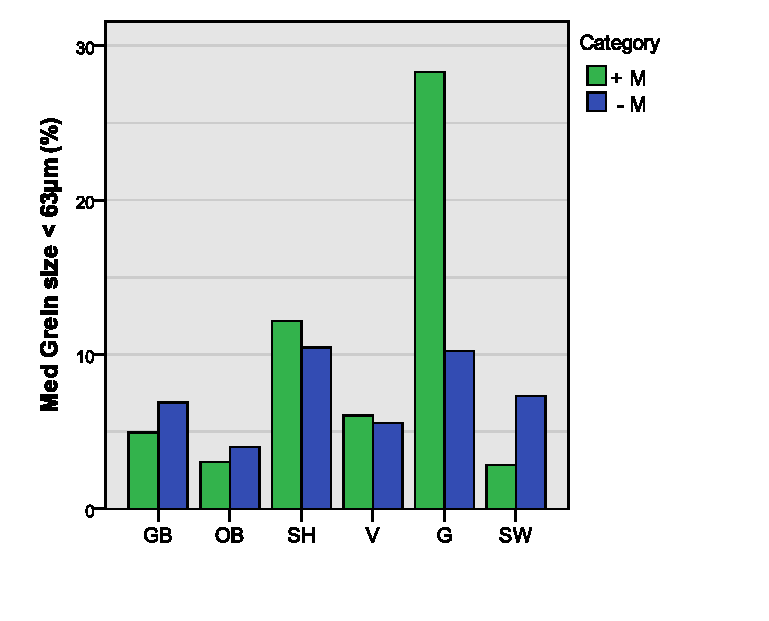
\includegraphics[width=0.75\textwidth]{images/salzsedimentauswertung/bar_63.eps}
\caption[Anteil der \unit{<63}{\mu\metre}-Korngrößenfraktion an Stationen des Salzgradienten]{Anteil der \unit{<63}{\mu\metre}-Korngrößenfraktion an Stationen des Salzgradienten; GB = Geltinger Bucht, OB = Orther Bucht; SH = Salzhaff; V = Vitter Bodden (5.7.2013), G = Griebener Bucht (30.7.2013), SW = Spandowerhagener Wiek}
\label{fig:sg:kleiner_63}
\end{figure}

\begin{figure}[htb]
\centering
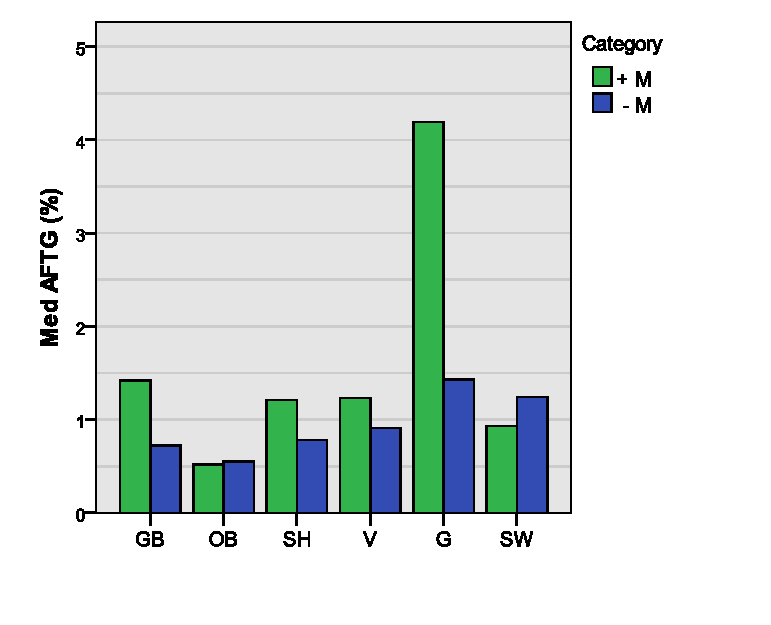
\includegraphics[width=0.75\textwidth]{images/salzsedimentauswertung/bar_aftg.eps}
\caption[Organischer Gehalt der Sedimente an Stationen des Salzgradienten]{Organischer Gehalt der Sedimente  an Stationen des Salzgradienten; GB = Geltinger Bucht, OB = Orther Bucht; SH = Salzhaff; V = Vitter Bodden (5.7.2013), G = Griebener Bucht (30.7.2013), SW = Spandowerhagener Wiek}
\label{fig:sg:afdg}
\end{figure}
\FloatBarrier

\subsubsection{Zusammenhänge zwischen Vegetation und Korngrößen}

Im Vergleich der Vegetation (Deckung und PVI) mit dem Median der Korngröße aller Standorte entlang des Salzgradienten ergibt sich keine lineare Abhängigkeit zwischen den Parametern (vgl. Abbildung \ref{fig: Regression_Vegetation_Korngroesse}). Das heißt es gibt keine tendenzielle Abnahme der Korngröße bei zunehmenden Deckungsgraden oder Anteilen der Vegetation an der Wassersäule. 

Werden alle Stationen einzeln betrachtet, fällt auf, dass der Median der Korngrößen, mit Ausnahme der Geltinger Bucht, an den spärlich bewachsenen Stellen um 0,1 bis 0,34 $ \Phi$-Einheiten niedriger, das Sediment also etwas grobkörniger ist (Vgl. Abbildung \ref{fig:sg:mittlere_kg}).

Auch beim Vergleich der feinsten Siebfraktion (\unit{<63}{\mu\metre}) mit den Vegetationsparametern Deckung und PVI ergibt sich keine lineare Beziehung (Vgl. Abbildung \ref{fig: Regression_Vegetation_63}). Im Vergleich zwischen dicht und spärlich besiedelten Untersuchungsgruppen ist ebenfalls kein Hinweis darauf zu finden, dass  es einen Zusammenhang zwischen dem Bewuchs mit Phytobenthos und dem Anteil der Ton/Siltfraktion gäbe. 



\begin{figure}[htb]
        \centering
        \begin{subfigure}[htb]{0.45\textwidth}
                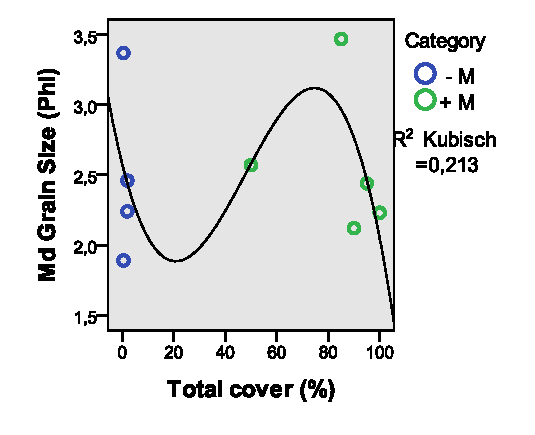
\includegraphics[width=\textwidth]{images/salzsedimentauswertung/gz_vs_cover.eps}
        \end{subfigure}
        \begin{subfigure}[htb]{0.45\textwidth}
                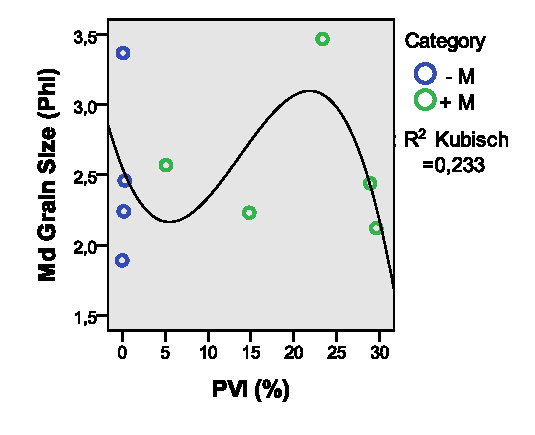
\includegraphics[width=\textwidth]{images/salzsedimentauswertung/gz_vs_pvi.eps}
        \end{subfigure}
        \caption[Regressionsmodell: Vegetation und Median der Korngröße für Stationen des Salzgradienten]												{Zusammenhang zwischen Median der Korngröße und den 																vegetationsbeschreibenden Parametern Deckung (links) und PVI (rechts) für 											Standorte entlang des Salzgradienten}
        \label{fig: Regression_Vegetation_Korngroesse}
\end{figure}

\begin{figure}[!htb]
        \centering
        \begin{subfigure}[htb]{0.45\textwidth}
                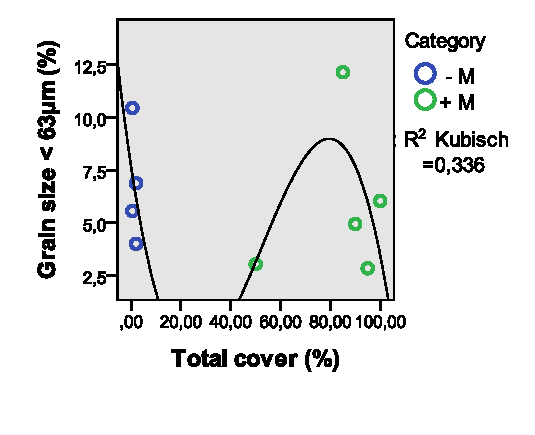
\includegraphics[width=\textwidth]{images/salzsedimentauswertung/63_vs_cover.eps}
        \end{subfigure}
        \begin{subfigure}[htb]{0.45\textwidth}
                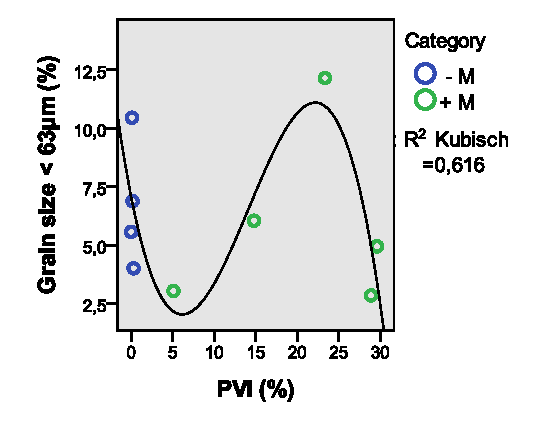
\includegraphics[width=\textwidth]{images/salzsedimentauswertung/63_vs_pvi.eps}
        \end{subfigure}
        \caption[Regressionsmodell: Vegetation und \unit{<63}{\mu\metre}-Korngrößenanteil für Stationen des 											Salzgradienten]{Zusammenhang zwischen \unit{<63}{\mu\metre}-Korngrößenanteil 									und den vegetationsbeschreibenden Parametern Deckung (links) und PVI 												(rechts) für Standorte entlang des Salzgradienten}
        \label{fig: Regression_Vegetation_63}
\end{figure}

\FloatBarrier

In Abbildung \ref{fig:matrixplot} sind verschiedene Parameter bzw. Prädikatoren (Salinität, Wassertiefe, Fetch, Cover, PVI) eingezeichnet, die einen Einfluss auf die mittlere Korngröße haben könnten. Es lässt sich bereits erkennen, dass keine der untersuchten Prädikatoren eine starke lineare Abhängigkeit zur mittleren Korngröße aufweist. Die Windlauflänge (Fetch) sowie die Salinität zeigen in einer Spearman-Rang-Korrelation die größten Abhängigkeiten mit Koeffizienten von -0,6 und 0,6, jedoch mit Irrtumswahrscheinlichkeiten von \unit{7-15}{\%}, dass heißt, diese Parameter könnten die mittlere Korngröße, im Gegensatz zu den Vegetationsparametern beeinflussen, jedoch reichen sie nicht aus, um das Vorhandensein bestimmter mittlerer Korngrößen zu erklären.


\begin{figure}[!htb]
\centering
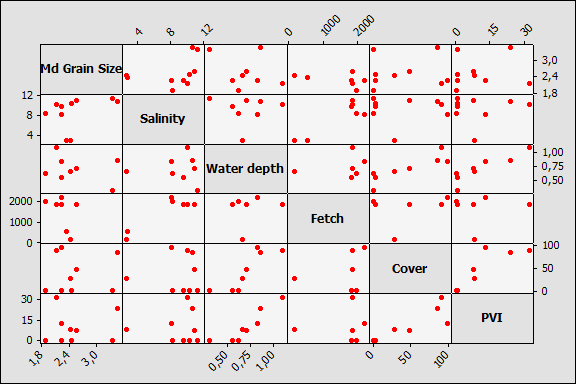
\includegraphics[width=0.75\textwidth]{images/matrixplot/Matrixplot_ohne_Grieben_neu2.png}
\caption[Korrelationsmatrix: Median der Korngröße und 5 Prädikatoren]{Korrelationsmatrix: Median der Korngröße und 5 Prädikatoren: Salinität, Wassertiefe, Fetch, Bedeckung mit Phytobenths und PVI}
\label{fig:matrixplot}
\end{figure}

\FloatBarrier


\begin{table}[!htb]
\centering
\caption[Spearman Rang-Korrelationen zur mittleren Korngröße entlang des Salzgradienten]{Spearman Rang-Korrelationen zur mittleren Korngröße entlang des Salzgradienten; 5 Prädikatoren: Salinität, Wassertiefe, Fetch, Bedeckung mit Phytobenthos, PVI}
\begin{tabular}{lrrrrr}

\toprule
& \multicolumn{5}{c}{Correlation / \textit{p}-Value} \\
\midrule
& \multicolumn{1}{c}{Md Grain Size}  & \multicolumn{1}{c}{Salinity} & \multicolumn{1}{c}{Water Depth} & \multicolumn{1}{c}{Fetch} & \multicolumn{1}{c}{Cover} \\

\midrule

Salinity        &       0,600\\
                &       0,067\\
\midrule
Water depth	    &     	-0,095           &-0,075\\
                &     	0,823            &0,860\\
\midrule
Fetch  	        &   	-0,608           &0,315            &0,371 \\
                &   	0,147            &0,491            &0,468 \\
\midrule
Cover  	        &     	-0,079           &-0,188           &0,888 		&0,282\\
                &     	0,840            &0,628            &0,003 		&0,589\\
\midrule
PVI	            &     	0,057            &-0,124           &0,915			&0,022            &0,924\\
                &     	0,884            &0,750            &0,001			&0,968            &0,000\\                    
\bottomrule

\end{tabular}
\label{tab:spearman_rank_correlations}
\end{table}



\begin{table}[!htb]
\centering
\caption[Schrittweise Regression: Median der Korngröße im Vergleich zu 4 Prädikatoren]{Schrittweise Regression (Rückwärts-Selektion, Alpha für Abnahme: 0,1, N = 6-10): Median der Korngröße im Vergleich zu Salinität, Wassertiefe, Fetch und PVI, die Bedeckung mit Phytobenthos wurde aufgrund der Korrelation zum PVI aus dem Modell entfernt}
\begin{tabular}{lrrrrr}

\toprule

Step    &        1 &     2   &   3    &  4    &  5\\
Constant &   4,509 & 5,093 & 5,636 & 7,157 & 4,000\\
\midrule

Salinity       &   0,52 &  0,42  & 0,42\\
T-Value    &  0,74  & 0,93 &  1,12\\
P-Value   &  0,594 & 0,452 & 0,345\\
\midrule
Water Depth     &   -0,8\\
T-Value   &  -0,29\\
P-Value   &  0,819\\
\midrule
Fetch       &  -0,56 & -0,83 & -0,83 & -0,73\\
T-Value   &  -0,46 & -1,45 & -1,75 & -1,51\\
P-Value   &  0,723 & 0,283 & 0,179 & 0,205\\
\midrule
PVI          &  0,66  & 0,11\\
T-Value     &0,33  & 0,25\\
P-Value     &0,795 & 0,823\\
\midrule
\midrule
S           & 3,69  & 2,72 &  2,25 &  2,32  & 2,61\\
$R^2$        &59,97 & 56,55 & 55,15 & 36,43  & -0,00\\
$R^2$(adjusted)    &\textbf{0,00}  & \textbf{0,00} & \textbf{25,25} & \textbf{20,54}   & \textbf{0,00}\\
Mallows Cp    &5,0    &3,1  &  1,1 &  -0,4   &-1,5\\
\bottomrule

\end{tabular}
\label{tab:spearman_rank_correlations}
\end{table}




\subsubsection{Zusammenhang zwischen Vegetation und organischem Gehalt der Sedimente}

Für die Standorte des Salzgradienten gibt es eine schwache Korrelation ($ Pearsson-R^2 = 0,56 $) zwischen dem Anteil der Pflanzen in der Wassersäule und dem organischen Gehalt der Sedimente. Der PVI zeigt einen größeren Einfluss auf den organischen Gehalt der Sedimente als die Bedeckung mit Makrophyten ($Pearsson-R^2 = 0,5$). Das heißt die Wuchshöhen und/ oder die Wassertiefe haben ebenfalls einen Einfluss (Vgl. Abbildung \ref{fig:sg:afdg_regressionen}). 
Das Regressionsmodell nach Spearman unter der Berücksichtigung der Prädikatoren Salinität, Wassertiefe, Fetch und Vegetation (Bedeckung mit Phytobenthos), zeigt, dass sich der organische Gehalt der Sedimente am Besten mit den Parametern Wassertiefe, Bedeckung mit Phytobentos und Salinität erklären lässt. Das Modell zeigt den besten Kompromiss zwischen geringer Prädikatorenaufnahme in das Modell (Mallow's Cp) und hohen korrigierten \textit{p}-Werten.

\begin{figure}[!htb]
\centering
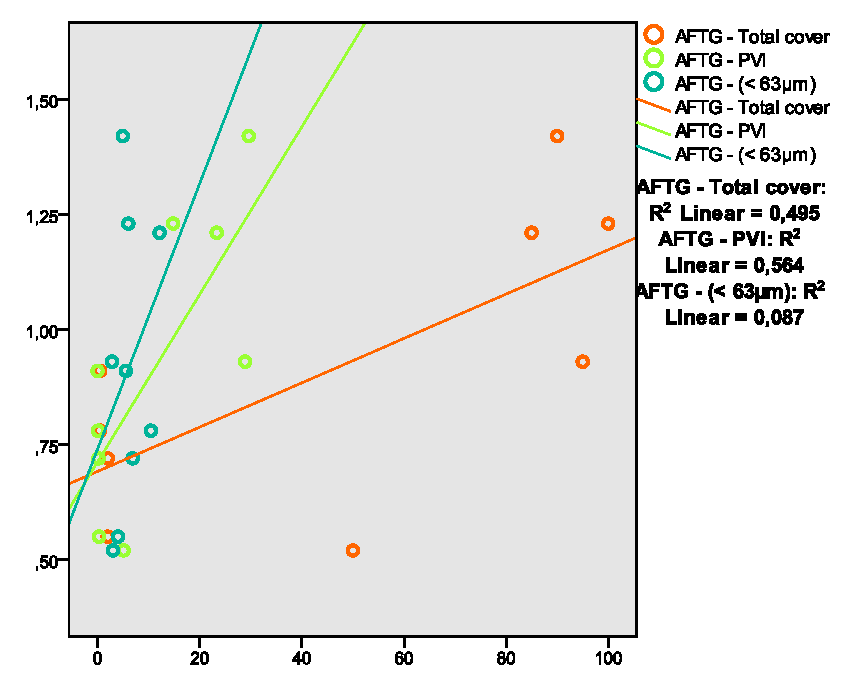
\includegraphics[width=0.75\textwidth]{images/salzsedimentauswertung/afdg1.eps}
\caption[Zusammenhang zwischen organischem Gehalt,\unit{<63}{\mu\metre}-Korngrößenfraktion und Vegetation]{Zusammenhang zwischen organischem Gehalt,\unit{<63}{\mu\metre}-Korngrößenfraktion und Vegetation (Deckung und PVI) an Stationen des Salzgradienten; GB = Geltinger Bucht, OB = Orther Bucht; SH = Salzhaff; V = Vitter Bodden (5.7.2013), G = Griebener Bucht (30.7.2013), SW = Spandowerhagener Wiek}
\label{fig:sg:afdg_regressionen}
\end{figure}

\begin{figure}[!htb]
\centering
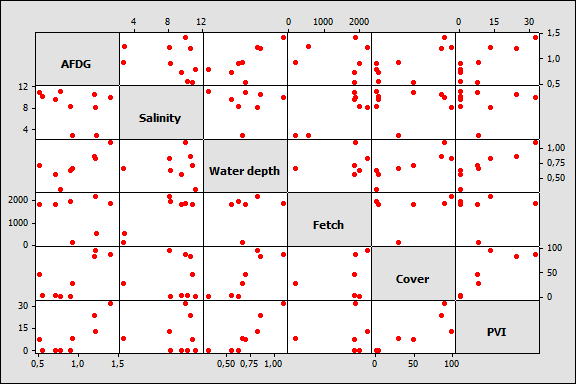
\includegraphics[width=0.75\textwidth]{images/matrixplot/afdg_matrixplot.png}
\caption[Korrelationsmatrix: Organischer Gehalt der Sedimente und 5 Prädikatoren]{Korrelationsmatrix: Median der Korngröße und 5 Prädikatoren ( Salinität, Wassertiefe, Fetch, Bedeckung mit Phytobenths und PVI)}
\label{fig:sg:afdg_matrixplot}
\end{figure}



\begin{table}[!htb]
\centering
\caption[Spearman Rang-Korrelationen zum organischen Gehalt der Sedimente]{Spearman Rang-Korrelationen zum organischen Gehalt der Sedimente (AFDG) entlang des Salzgradienten; 5 Prädikatoren: Salinität, Wassertiefe, Fetch, Bedeckung mit Phytobenthos, PVI}
\begin{tabular}{lrrrrr}

\toprule
& \multicolumn{5}{c}{Correlation / \textit{p}-Value} \\
\midrule
& \multicolumn{1}{c}{AFDG}  & \multicolumn{1}{c}{Salinity} & \multicolumn{1}{c}{Water Depth} & \multicolumn{1}{c}{Fetch} & \multicolumn{1}{c}{Cover} \\

\midrule

Salinity        &       -0,491\\
                &       0,150\\
\midrule
Water depth	    &     	0,669  			&-0,075\\
        		&		0,070   		&0,860\\
\midrule
Fetch  	        &   	0,118   		&0,315			   &0,371\\
        		&		0,801  			&0,491   			&0,468 \\
\midrule
Cover  	        &     	0,596  			&-0,188   			&0,888   		&0,282\\
        		&		0,090   		&0,628   			&0,003   		&0,589\\
\midrule
PVI	            &     	0,669  			&-0,124   			&0,915   		&0,022  	& 0,924\\
        		&		0,049   		&0,750   			&0,001   		&0,968   	&0,000\\
\bottomrule

\end{tabular}
\label{tab:spearman_rank_correlations_afdg}
\end{table}




\begin{table}[!htb]
\centering
\caption[Schrittweise Regression: Organischer Gehalt der Sedimente im Vergleich zu 4 Prädikatoren]{Schrittweise Regression (Rückwärts-Selektion, Alpha für Abnahme: 0,1, N = 4-10): Median der Korngröße im Vergleich zu Salinität, Wassertiefe, Fetch und Bedeckung mit Phytobenthos, das PVI  wurde aufgrund der Korrelation zum PVI und zur Wassertiefe aus dem Modell entfernt}
\begin{tabular}{lrrr}
\toprule
Step      	&     1  &    2     & 		3\\
Constant   	& 2,895  &	3,519  	&	3,231\\
\midrule
Salinity         & -0,81  &	-0,78  	&	-0,74\\
T-Value     & -1,93  &	-2,39  	&	-2,55\\
P-Value     & 0,305  &	0,139  	&	0,084\\
\midrule
Water depth       & 1,56   &	1,67   	&	1,23\\
T-Value     & 1,55   &	2,17   	&	3,34\\
P-Value     &0,364  &	0,162  	&	0,044\\
\midrule
Fetch       &   0,27\\
T-Value    &  0,49\\
P-Value    & 0,711\\
\midrule
Cover      &   -0,38  &	-0,40\\
T-Value   &  -0,51  &	-0,68\\
P-Value   &  0,700  &	0,568\\
\midrule
\midrule
S        &    2,44   &	1,92   	&	1,74\\
$R^2$      &  88,85  &	86,20  	&	83,04\\
$R^2$(adjusted) &  44,26  &	65,50  	&	71,73\\
Mallows Cp  &  5,0  &  	3,2    	&	1,5 \\
\bottomrule
\end{tabular}
\label{tab:spearman_rank_correlations}
\end{table}








   